\chapter{群速度、费米子排斥与狄拉克海}

\section{相速度与群速度}

\begin{classroomqa}
\lecturetimestamp{00:00:07}
\audiencequestion{什么是群速度和相速度？}
\lecturerresponse{相速度跟随平面波中相位固定的一个点。它通常并不描述可测量物体的运动。群速度跟随波包的包络，是与粒子、信号和概率流相关联的速度。}
\end{classroomqa}

从平面波开始，
\begin{equation}
\psi(x,t)=e^{i(kx-\omega t)},
\end{equation}
或者用它的实形式，
\begin{equation}
\psi(x,t)=\sin(kx-\omega t).
\end{equation}
一个波峰、一个波谷，或任何其他相位固定的点，其移动满足
\begin{equation}
kx-\omega t=\text{constant}.
\end{equation}
为方便起见取该常数为零，得到
\begin{equation}
x=\frac{\omega}{k}t,
\qquad
v_{\mathrm{phase}}=\frac{\omega}{k}.
\end{equation}
由于\(\omega=2\pi/T\)和\(k=2\pi/\lambda\)，
\begin{equation}
v_{\mathrm{phase}}=\frac{\omega}{k}=\frac{\lambda}{T}.
\end{equation}
这不过是一个给定相位在一个周期内前进的距离。

对于非相对论性的Schr\"odinger波，取\(\hbar=1\)，能量和动量为\(\omega\)和\(k\)，因此
\begin{equation}
\omega(k)=\frac{k^2}{2m}.
\end{equation}
其相速度因此为
\begin{equation}
v_{\mathrm{phase}}=\frac{k}{2m}.
\end{equation}
然而，动量为\(k\)的粒子的通常速度为\(k/m\)。这个两倍的差异是第一个警告：平面波相位的运动并不是粒子的运动。

还有一个更尖锐的警告。给每个频率加上同一个常数\(C\)：
\begin{equation}
\omega(k)\longrightarrow \omega(k)+C.
\end{equation}
这个常数例如可以代表一个共同的静止能量贡献，如\(mc_{\mathrm{light}}^2\)，但它的具体名称并不重要。这里\(C\)是能量偏移，而不是光速。相速度变为
\begin{equation}
v_{\mathrm{phase}}\longrightarrow
\frac{\omega(k)+C}{k}
=v_{\mathrm{phase}}+\frac{C}{k}.
\end{equation}
然而，给每个能量加上同一个常数并不改变任何能量差，因此也不改变任何非相对论物理。

这可以直接在波函数中看出。将一般的Schr\"odinger场写成模式的求和或积分，
\begin{equation}
\psi(x,t)=\sum_k a_k e^{ikx}e^{-i\omega(k)t},
\end{equation}
其中归一化因子被省略。在平移之后，
\begin{align}
\psi(x,t)
&\longrightarrow
\sum_k a_k e^{ikx}e^{-i[\omega(k)+C]t}
\\
&=e^{-iCt}\psi(x,t).
\end{align}
每个模式都获得了相同的时间相关相位。共轭场获得相反的相位，因此
\begin{equation}
\begin{aligned}
\psi^*(x,t)\psi(x,t)
&\longrightarrow
e^{iCt}e^{-iCt}\psi^*(x,t)\psi(x,t)
\\
&=\psi^*(x,t)\psi(x,t).
\end{aligned}
\end{equation}
同样的抵消也发生在期望值中。一个在能量零点平移时会发生变化的量，不可能是Schr\"odinger粒子的物理传播速度。因此相速度部分是约定性的。

局域化的粒子不是由一个无限平面波表示，而是由一个波包表示。各分量波在波包区域内相长叠加，在区域外相消叠加。这个图案的运动已经可以从两个邻近的波求出：
\begin{equation}
\psi(x,t)=
\sin(kx-\omega t)+
\sin(k'x-\omega't),
\end{equation}
其中\(k'\)接近\(k\)，且\(\omega'=\omega(k')\)。相长干涉的一个轨迹出现在它们的相位一致之处，
\begin{equation}
kx-\omega t=k'x-\omega't.
\end{equation}
因此
\begin{equation}
(k-k')x=(\omega-\omega')t,
\end{equation}
而增强图案按照下式移动
\begin{equation}
x=\frac{\omega-\omega'}{k-k'}t.
\end{equation}
取邻近波的极限得到
\begin{equation}
x=\frac{d\omega}{dk}t,
\qquad
v_{\mathrm{group}}=\frac{d\omega}{dk}.
\end{equation}
这就是包络的速度---即由各分量波干涉产生的局域团块的速度。

对于非相对论色散关系，包括任意偏移，
\begin{equation}
\omega(k)=\frac{k^2}{2m}+C,
\end{equation}
群速度为
\begin{equation}
v_{\mathrm{group}}
=\frac{d}{dk}\left(\frac{k^2}{2m}+C\right)
=\frac{2k}{2m}
=\frac{k}{m}.
\end{equation}
加性常数已经消失，结果正是经典粒子速度。

\begin{classroomqa}
\lecturetimestamp{00:16:35}
\audiencequestion{两倍的因子在群速度中会消失吗？}
\lecturerresponse{会。对\(k^2\)求导产生\(2k\)，它抵消了\(2m\)中的2。结果是\(k/m\)。}
\end{classroomqa}

因此，群速度是与经典粒子运动联系最紧密的速度。它也是与波包传播相关的速度，并且在这里所考虑的通常情形下，与信号传播相关。相速度则不必具有这两种含义中的任何一种。

\subsection{无质量与有质量的相对论性波}

\begin{classroomqa}
\lecturetimestamp{00:17:47}
\audiencequestion{这与光可以比光传播得更快的说法有关吗？}
\lecturerresponse{没有。那些说法提出了一个单独的问题。一个相关的计算确实表明，相位可以比光移动得更快，而物理的群速度仍然保持亚光速，但这并不描述一个超过光的信号。}
\end{classroomqa}

\begin{classroomqa}
\lecturetimestamp{00:18:05}
\audiencequestion{相关的例子是不是那个熟悉的例子：相速度超过光速，而群速度仍低于它？}
\lecturerresponse{是的。同样的模式出现在具有非零质量的相对论性波中，并且它直接来自相对论能量--动量关系。}
\end{classroomqa}

设 \(\hbar=c_{\mathrm{light}}=1\)。相对论关系为
\begin{equation}
E=\sqrt{p^2+m^2},
\qquad
\omega(k)=\sqrt{k^2+m^2}.
\end{equation}
先确立无质量情形是有用的。当 \(m=0\) 时，
\begin{equation}
\omega=|k|.
\end{equation}
在右行支 \(k>0\) 上，\(\omega=k\)，因此
\begin{equation}
v_{\mathrm{phase}}=\frac{\omega}{k}=1,
\qquad
v_{\mathrm{group}}=\frac{d\omega}{dk}=1.
\end{equation}
在左行支上，两个速度都取相应的负号。无论哪种情形，它们的速率都是光速。由于色散关系在任一支上都是线性的，该支上的所有傅里叶分量都以同一速度运动。

对于 \(k>0\) 的有质量粒子，
\begin{equation}
v_{\mathrm{phase}}
=\frac{\omega}{k}
=\sqrt{\frac{k^2+m^2}{k^2}}>1,
\end{equation}
而
\begin{equation}
v_{\mathrm{group}}
=\frac{d\omega}{dk}
=\frac{k}{\sqrt{k^2+m^2}}<1.
\end{equation}
对于 \(k<0\)，两个速度都反号，而它们的大小满足同样的不等式。因此，相位可以比光运动得更快，而波包、粒子、能量和信号则比光运动得更慢。对于这一特定的色散关系和 \(k\neq0\)，
\begin{equation}
v_{\mathrm{phase}}v_{\mathrm{group}}=1.
\end{equation}
这一反比关系是平方根色散关系的偶然结果，而不是波的一般性质。

\begin{figure}
\centering
\includegraphics[width=0.72\textwidth]{lecture_05_figure_03.png}
\caption{非相对论与相对论色散关系，其中相速度为 \(\omega/k\)，群速度为 \(d\omega/dk\)。}
\lectureframe{00:35:52}
\end{figure}

\begin{classroomqa}
\lecturetimestamp{00:23:41}
\audiencequestion{色散是否与波速依赖于频率有关？}
\lecturerresponse{是的。当 \(\omega(k)\) 为线性时，每个傅里叶分量都具有相同的群速度，波包可以保持其形状。当 \(\omega(k)\) 为非线性时，不同分量以不同速度运动，因此波包发生色散并改变形状。低频声在频率近似正比于波数时近似为非色散的。}
\end{classroomqa}

相速度通常既不携带信号，也不携带能量，也不携带概率流。它的数值甚至可以通过移动能量零点而改变。群速度是足够窄的波包在物理上相关的运动。

\begin{classroomqa}
\lecturetimestamp{00:25:14}
\audiencequestion{光子的相速度可以被测量吗？}
\lecturerresponse{在真空中，光子具有线性色散，因此其相速度和群速度重合，二者都等于光速。在物质介质中，色散关系改变，相速度和群速度不必一致。}
\end{classroomqa}

\begin{classroomqa}
\lecturetimestamp{00:25:50}
\audiencequestion{这一讨论是否仅限于不随时间展宽的波包？}
\lecturerresponse{只有当波包的所有傅里叶分量都具有同一速度时，波包才保持不展宽，这对应于相关范围内线性的色散关系。对于非线性色散，各分量分离，波包展宽。}
\end{classroomqa}

关于光锥和相对论因果结构的问题所需的讨论超出了相速度与群速度之间的区分，因此与这一计算分开处理。

\section{平移对称性与守恒定律}

同样的平面波相位可以简洁地说明守恒定律。从能量守恒开始。一个湮灭场作用于能量为 \(\omega_j\) 的入射粒子，贡献一个时间因子
\begin{equation}
e^{-i\omega_j t},
\end{equation}
而一个产生能量为 \(\omega'_r\) 的出射粒子的产生场贡献
\begin{equation}
e^{+i\omega'_r t}.
\end{equation}
对于若干入射粒子和出射粒子，它们的乘积为
\begin{equation}
\exp\!\left[
i\left(\sum_r\omega'_r-\sum_j\omega_j\right)t
\right].
\end{equation}
如果相互作用可以在任意时刻以相同振幅发生，则振幅包含对相互作用时间的积分：
\begin{equation}
\begin{aligned}
&\int_{-\infty}^{\infty}dt\,
\exp\!\left[
i\left(\sum_r\omega'_r-\sum_j\omega_j\right)t
\right]
\\
&\quad =2\pi\,
\delta\!\left(\sum_r\omega'_r-\sum_j\omega_j\right).
\end{aligned}
\end{equation}
{\proseunicodefont δ}函数要求出射总能量等于入射总能量。在每个可能的相互作用时刻振幅都相同，就是时间平移不变性，它产生能量守恒。

空间平移通过同样的机制给出动量守恒。考虑一个物理的一变二衰变，其中动量为\(k\)的入射粒子消失，而动量为\(k'_1\)和\(k'_2\)的两个粒子出现。位于位置\(x\)处的局域相互作用包含一个湮灭场和两个产生场，
\begin{equation}
\mathcal{O}(x)=\psi^\dagger(x)\psi^\dagger(x)\psi(x).
\end{equation}
忽略时间依赖性和归一化，相关的模式因子为
\begin{align}
\psi(x)&\supset a_k e^{ikx},
\\
\psi^\dagger(x)&\supset a_{k'_1}^\dagger e^{-ik'_1x},
\qquad
\psi^\dagger(x)\supset a_{k'_2}^\dagger e^{-ik'_2x}.
\end{align}
在矩阵元
\begin{equation}
\langle k'_1,k'_2|\mathcal{O}(x)|k\rangle,
\end{equation}
中，湮灭算符移除入射粒子，而两个产生算符提供出射粒子。一旦完成了这些算符作用，剩余的位置相关因子为
\begin{equation}
e^{-ik'_1x}e^{-ik'_2x}e^{ikx}
=e^{i(k-k'_1-k'_2)x}.
\end{equation}
由于没有任何位置是特殊的，需要对所有可能的衰变位置积分：
\begin{equation}
\int_{-\infty}^{\infty}dx\,
e^{i(k-k'_1-k'_2)x}
=2\pi\delta(k-k'_1-k'_2).
\end{equation}
因此，幸存的振幅满足
\begin{equation}
k=k'_1+k'_2.
\end{equation}
在三维中，同样的计算使用\(d^3x\)、粗体动量矢量和三维{\proseunicodefont δ}函数。论证中没有任何内容依赖于只有一个入射粒子或两个出射粒子。对于任意粒子数，对共同相互作用位置积分给出
\begin{equation}
\delta^{(3)}\!\left(
\sum_j\mathbf{k}_j-\sum_r\mathbf{k}'_r
\right).
\end{equation}
每个位置处振幅相等就是空间平移不变性，它正如每个时刻振幅相等给出能量守恒一样，给出动量守恒。

第三个例子是整体相位旋转，
\begin{equation}
\psi\longrightarrow e^{i\lambda}\psi,
\qquad
\psi^\dagger\longrightarrow e^{-i\lambda}\psi^\dagger.
\end{equation}
当一个相互作用振幅中湮灭场和产生场贡献的相位相互抵消时，该振幅是不变的。对于携带电荷的场，从初态移除的电荷与在末态恢复的电荷之间的这种相等就是电荷守恒。因此，时间平移、空间平移和整体相位旋转说明了产生和湮灭粒子的场如何编码能量、动量和电荷守恒。

\begin{classroomqa}
\lecturetimestamp{00:37:52}
\audiencequestion{对空间积分是指对所有三个空间维度积分吗？}
\lecturerresponse{是的。这三个积分产生一个关于三个动量分量的{\proseunicodefont δ}函数，因此总动量的所有三个分量都守恒。}
\end{classroomqa}

\begin{classroomqa}
\lecturetimestamp{00:38:03}
\audiencequestion{这个模型是否决定了以不同方式分配守恒动量的相对概率？}
\lecturerresponse{不。这个简单的表达式强制了出射动量之和，但除此之外对它们的分配保持中立。相对概率需要额外的动力学信息。}
\end{classroomqa}

\begin{classroomqa}
\lecturetimestamp{00:39:04}
\audiencequestion{为什么湮灭算符之和会约化为与占据动量匹配的那一项？}
\lecturerresponse{湮灭算符作用于空模式给出零矢量。如果态中只有一个粒子且位于模式\(k_0\)中，那么除了带有\(k=k_0\)的那一项之外，每一项都消失。}
\end{classroomqa}

例如，
\begin{equation}
\sum_k a_k e^{ikx}|1_{k_0}\rangle
=e^{ik_0x}|0\rangle,
\end{equation}
在归一化意义下：所有与空模式相关的湮灭算符都返回零矢量。

\section{玻色增强与费米排斥}

玻色子允许单粒子态中任意非负的占据数，而且它们的产生算符代数实际上偏好已经被占据的态。对于一个玻色模式，归一化的数态约定将占据增强写为\footnote{讲义陈述了平方根占据增强；这个带编号的方程是其标准的数态形式。}
\begin{equation}
a^\dagger|n\rangle=\sqrt{n+1}\,|n+1\rangle.
\end{equation}
假设一个激发态原子可以向许多可能的模式发射一个光子。在不存在其他光子的情况下，不同方向和动量以其通常的概率分布出现。如果某个特定模式已经包含许多光子---全都具有相同的动量、能量和频率---，那么向该模式的发射会被相应的平方根占据因子增强。原子优先将其光子添加到已经布居的态中。这就是受激发射，是玻色子聚集的一个具体表现。

费米子的行为相反。两个全同费米子不能占据同一个量子态。泡利不相容原理最初出现在原子物理中，在那里原子中的两个电子不能具有完全相同的量子数，但它并不局限于原子：在任何地方，全同费米子都不能共享一个完整的单粒子态。

场的展开最初看起来与玻色子的展开完全一样。在有限盒子中，可以写出
\begin{equation}
\psi(x)=\sum_k A_k e^{ikx},
\qquad
\psi^\dagger(x)=\sum_k A_k^\dagger e^{-ikx}.
\end{equation}
对于连续动量，求和变为积分。共轭空间相位中的相反符号来自厄米共轭。构造的这一部分是非相对论性的；相对论性费米子只会在最后进入。

场的状态仍然由每个模式的占据数来记录，但现在每个数只能为零或一：
\begin{equation}
|n_{k_1},n_{k_2},\ldots\rangle,
\qquad n_k\in\{0,1\}.
\end{equation}
不存在额外的相对论性粒子类型，例如每个状态至多三个粒子或每个状态至少七个粒子。要确立玻色统计和费米统计是仅有的可能性，需要量子力学与狭义相对论相结合，这超出了目前的讨论范围。这里的任务是描述费米子可能性及其后果。

\subsection{一个费米子态}

聚焦于单个单粒子态。它要么是空的，\(|0\rangle\)，要么是被占据的，\(|1\rangle\)。产生和湮灭算符的作用为
\begin{align}
A^\dagger|0\rangle&=|1\rangle,
&
A^\dagger|1\rangle&=0,
\\
A|0\rangle&=0,
&
A|1\rangle&=|0\rangle.
\end{align}
右侧不带修饰的零是零矢量，而不是空态\(|0\rangle\)。试图加入第二个费米子并不会返回真空；它根本不返回任何物理态。

\begin{classroomqa}
\lecturetimestamp{00:46:25}
\audiencequestion{费米子的产生和湮灭算符仍然是线性的吗？}
\lecturerresponse{是的。量子力学算符是线性算符，费米子的产生和湮灭算符也包括在内。}
\end{classroomqa}

\begin{classroomqa}
\lecturetimestamp{00:47:34}
\audiencequestion{零是指空态，还是指所尝试的操作无法产生一个态？}
\lecturerresponse{它指的是零矢量，而不是空态。真正的真空或基态具有非零波函数；恒为零的函数具有零范数，不是物理态。}
\end{classroomqa}

谐振子使这一区分变得具体。它的基态，即没有振子激发的态，具有诸如
\begin{equation}
\phi_0(q)\propto e^{-\alpha q^2},
\qquad \alpha>0.
\end{equation}
这样的高斯波函数。这是一个完全良好、可归一化的态。相比之下，
\begin{equation}
\phi(q)\equiv0
\end{equation}
是零矢量：它在任何地方都没有概率幅，不是一个态。因此\(A^\dagger|1\rangle=0\)表明，所尝试的第二次产生给出的是零矢量。

\begin{classroomqa}
\lecturetimestamp{00:48:42}
\audiencequestion{费米子算符是否应使用与玻色子算符不同的记号？}
\lecturerresponse{是的。将\(a\)和\(a^\dagger\)保留给玻色模式，而用\(c\)和\(c^\dagger\)表示费米模式，会更加清楚。两种约定在文献中都出现过，但使用不同的字母能使这两种代数保持区分。}
\end{classroomqa}

采用该记号后，单模式规则为
\begin{align}
c^\dagger|0\rangle&=|1\rangle,
&c^\dagger|1\rangle&=0,
\\
c|0\rangle&=0,
&c|1\rangle&=|0\rangle.
\end{align}
现在在两个基态上计算两种可能的乘积。在空态上，
\begin{align}
c^\dagger c|0\rangle&=0,
&
cc^\dagger|0\rangle&=|0\rangle.
\end{align}
在占据态上，
\begin{align}
c^\dagger c|1\rangle&=|1\rangle,
&
cc^\dagger|1\rangle&=0.
\end{align}
它们的和返回它所作用的那个态：
\begin{align}
(c^\dagger c+cc^\dagger)|0\rangle&=|0\rangle,
\\
(c^\dagger c+cc^\dagger)|1\rangle&=|1\rangle.
\end{align}
由于\(|0\rangle\)和\(|1\rangle\)张成单模式态空间，
\begin{equation}
c^\dagger c+cc^\dagger=1.
\end{equation}
带正号的组合是反对易子，
\begin{equation}
\{A,B\}=AB+BA,
\end{equation}
因此费米子关系为
\begin{equation}
\{c,c^\dagger\}=1.
\end{equation}
它是玻色子对易子
\begin{equation}
[a,a^\dagger]=aa^\dagger-a^\dagger a=1.
\end{equation}
的费米子类比。

在同一费米子态中的两次产生总是为零。如果该态是空的，第一次产生将其填满，第二次则失败；如果它已被占据，第一次产生就已经失败。类似地，两次湮灭总是为零。因此
\begin{equation}
\{c^\dagger,c^\dagger\}=2(c^\dagger)^2=0,
\qquad
\{c,c\}=2c^2=0.
\end{equation}

\begin{classroomqa}
\lecturetimestamp{00:56:45}
\audiencequestion{平方湮灭关系中的零是零矢量吗？}
\lecturerresponse{该方程表明\(c^2\)是零算符。它是一个把每个态矢量都送到零矢量的算符。零算符和零矢量是不同的数学对象，尽管前者总是产生后者。}
\end{classroomqa}

对于许多离散动量模式，完整的代数为
\begin{align}
\{c_k,c_{k'}^\dagger\}&=\delta_{kk'},
\\
\{c_k,c_{k'}\}&=0,
\\
\{c_k^\dagger,c_{k'}^\dagger\}&=0.
\end{align}
克罗内克{\proseunicodefont δ}在\(k=k'\)时为一，否则为零。对于连续动量，在适当的归一化下，它被狄拉克{\proseunicodefont δ}函数取代。同类型的反对易子对每一对模式都为零，而不仅是在它们的标记相同时。

\subsection{位置空间中的排除}

以动量标记的代数首先表明，同一物种的两个全同费米子不能占据一个动量模式。它还表明更多内容。定域在位置\(x\)处的一个粒子由
\begin{equation}
\psi^\dagger(x)=\sum_k c_k^\dagger e^{-ikx},
\end{equation}
产生，至多相差一个归一化因子。在原点处，试图产生两个粒子给出
\begin{align}
\psi^\dagger(0)\psi^\dagger(0)|\Omega\rangle
&=\sum_{k,k'}c_k^\dagger c_{k'}^\dagger|\Omega\rangle.
\end{align}
标记\(k\)和\(k'\)是哑求和变量。交换它们不改变双重求和，因此可以与其重新标记后的形式取平均：
\begin{align}
\sum_{k,k'}c_k^\dagger c_{k'}^\dagger|\Omega\rangle
&=\frac12\sum_{k,k'}
\left(c_k^\dagger c_{k'}^\dagger
+c_{k'}^\dagger c_k^\dagger\right)|\Omega\rangle
\\
&=\frac12\sum_{k,k'}
\{c_k^\dagger,c_{k'}^\dagger\}|\Omega\rangle
=0.
\end{align}

\begin{classroomqa}
\lecturetimestamp{01:02:26}
\audiencequestion{在两粒子位置态求和中，是否只有动量不相等的项才为零？}
\lecturerresponse{不是。重新标记哑指标会把整个双重求和变成两个产生算符的反对易子的一半。该反对易子对每一对动量都为零，因此整个求和为零。}
\end{classroomqa}

计算表明，排斥并非动量本征态所特有。全同费米子也不能被置于相同的位形状态。更一般地说，它们不能占据任何相同的单粒子态。

\subsection{什么构成同一状态？}

\begin{classroomqa}
\lecturetimestamp{01:04:30}
\audiencequestion{两个相距很远的电子可以具有相同的动量吗？}
\lecturerresponse{排斥涉及的是完整的单粒子态。当另一个对易标签（例如自旋）不同时，两个电子可以具有完全相同的动量本征值。空间上分离的电子则是局域化波包，而非精确的动量本征态；它们的平均动量可以几乎相等，而空间波函数仍然不同。被禁止的是完整状态的相等。}
\end{classroomqa}

自旋尚未展开讨论，但它提供了一个熟悉的额外标签。当两个电子的自旋态不同时，它们可以共享相同的动量值。一旦把所有相关标签都包括进来，就没有两个全同费米子可以共享同一个完整状态。

\begin{classroomqa}
\lecturetimestamp{01:05:25}
\audiencequestion{两个分离氢原子中的电子可以具有相同的动量或原子状态吗？}
\lecturerresponse{束缚在原子中的电子不是动量本征态。它的轨道波函数以该原子为中心。两个分离的原子可以各有一个电子处于所谓的原子基态，但一个轨道以第一个原子为中心，另一个以第二个原子为中心，因此它们是不同的单粒子态。}
\end{classroomqa}

\begin{classroomqa}
\lecturetimestamp{01:06:33}
\audiencequestion{更一般的词“系统”可以替代“状态”吗？}
\lecturerresponse{不可以。系统是自由度的集合；状态则指定该系统的某一特定量子位形。电子是一个系统，而它的轨道与自旋波函数描述的是该系统的状态。}
\end{classroomqa}

\begin{figure}
\centering
\includegraphics[width=0.74\textwidth]{lecture_05_figure_04.png}
\caption{局域化单粒子波函数与用于检验费米子排斥的两个产生算符态。}
\lectureframe{01:07:21}
\end{figure}

\begin{classroomqa}
\lecturetimestamp{01:07:22}
\audiencequestion{阴极射线管中的电子流是否不包含两个处于同一状态的电子？}
\lecturerresponse{是的。这些电子占据不同的波包，它们在位置上分离，或者其完整状态以其他方式彼此区分。这与光子形成对比，光子可以全部占据同一个平面波模式并构成相干光束。}
\end{classroomqa}

电子束可以描绘为一个局域化波包接着另一个局域化波包。这些波包不必是精确的位置态或精确的动量态；只要它们的波函数彼此不同就够了。相比之下，光子束可以有许多光子处于完全相同的平面波态。

\begin{classroomqa}
\lecturetimestamp{01:08:14}
\audiencequestion{两个电子可以处于同一位置而具有不同动量吗？}
\lecturerresponse{精确位置和精确动量是不相容的标签，因为相应的算符不对易。人们不能通过同时具有确定位置和确定动量来指定一个单粒子态。自旋可以伴随位置标签或动量标签，因为在这种非相对论情形下自旋与那些可观测量对易。}
\end{classroomqa}

\begin{classroomqa}
\lecturetimestamp{01:08:51}
\audiencequestion{分离的束缚电子近似处于位置态吗？}
\lecturerresponse{它们不是精确的位置本征态，因为每个轨道都有有限的空间延展，但每个都近似局域化在各自的原子附近。这种局域化足以使两个轨道波函数成为不同的状态。}
\end{classroomqa}

\begin{classroomqa}
\lecturetimestamp{01:09:31}
\audiencequestion{量子状态的定义是什么？}
\lecturerresponse{状态是系统位形的量子类比。它包含为可能测量赋予概率所需的信息。对于一个电子，状态由波函数表示，并连同任何内部标签（例如自旋）一起表示。}
\end{classroomqa}

\begin{classroomqa}
\lecturetimestamp{01:10:32}
\audiencequestion{局域化在非常遥远地方的电子可以处于同一状态或具有相同动量吗？}
\lecturerresponse{它们不能是同一状态，因为它们的局域化不同：这里的一个电子和仙女座星系中的一个电子，或者内华达州的一个和康涅狄格州的一个，具有不同的波函数。它们可以具有几乎相等的动量。使任一动量无限确定都会使相应的波函数在空间中扩展，并破坏曾区分这些状态的局域化。}
\end{classroomqa}

位置--动量不确定性关系的标准差形式为\footnote{讲座给出了定性的不确定性乘积陈述；因子\(\hbar/2\)是在标准差约定下给出的。}
\begin{equation}
\Delta x\,\Delta p\geq\frac{\hbar}{2}.
\end{equation}
一个波包可以局域在内华达州，并具有相当窄的动量分布，而另一个在康涅狄格州的波包具有几乎相同的分布。它们仍然是不同的态，因为它们的空间波函数不同。在精确的动量本征极限下，两个波包都不再局域在任一地点。

费米子算符在反应中的使用方式与玻色子算符相同。电子湮灭算符移除一个入射电子，电子产生算符提供一个出射电子，这些因子可以与光子产生或湮灭算符相乘。光子是玻色子，而电子是费米子。它们算符的乘积为涉及入射和出射电子以及发射或吸收光子的反应提供了记账。

\begin{classroomqa}
\lecturetimestamp{01:13:36}
\audiencequestion{泡利不相容是局域传递的，还是在两个产生过程空间分离时全局强制执行的？}
\lecturerresponse{如果一个粒子已知在内华达州，另一个在康涅狄格州，那么它们不在同一个态中。}
\end{classroomqa}

\editorialnote{对这个问题的回答有一小部分无法恢复。局域单粒子态与内华达--康涅狄格叠加态之间的区别是可靠的。}

当它们的位置不确定时，不相容性要求判断完整的单粒子波函数是否重合。内华达--康涅狄格叠加态使这一区别变得明确。

设\(|N\rangle\)和\(|C\rangle\)为分别局域在内华达州和康涅狄格州的正交归一态。那么
\begin{equation}
|+\rangle=\frac{|N\rangle+|C\rangle}{\sqrt2},
\qquad
|-\rangle=\frac{|N\rangle-|C\rangle}{\sqrt2}.
\end{equation}
态\(|+\rangle\)给出在其一个电子在内华达州或康涅狄格州被找到的相等概率。态\(|-\rangle\)给出相同的位置概率，但相差一个相对相位。这两个态是正交的：
\begin{equation}
\langle+|-\rangle=0.
\end{equation}
两个电子不能同时占据\(|+\rangle\)，也不能同时占据\(|-\rangle\)，但不相容性并不阻止一个电子占据每个态。

\begin{classroomqa}
\lecturetimestamp{01:16:25}
\audiencequestion{一个电子可以占据加型内华达--康涅狄格叠加态，而另一个占据减型叠加态吗？}
\lecturerresponse{可以。加型和减型组合是正交的，因此是不同的单粒子态。}
\end{classroomqa}

\begin{classroomqa}
\lecturetimestamp{01:16:39}
\audiencequestion{分离态的例子需要同时性的概念吗？}
\lecturerresponse{目前的模型是非相对论性的。它在一个共同的时间切片上比较两个被占据的态，具有空间分离的内华达州和康涅狄格州区域共享的绝对时间。它还忽略了比较这些区域时有限速度的操作限制。相对论物理学在粒子如何局域化方面引入了额外的模糊性，但并未推翻不相容性，不过这一改进在此被推迟。}
\end{classroomqa}

本质性的非相对论陈述现在已确定：费米子由反对易的产生和湮灭算符描述，没有两个全同费米子能占据一个完整的单粒子态。因此多体基态与玻色子的基态截然不同。

\section{有限盒子中的玻色子和费米子基态}

考虑粒子被限制在边长为\(L\)的有限三维盒子中，具有周期性边界条件。在一维中，允许的波数为
\begin{equation}
k=\frac{2\pi n}{L},
\qquad n\in\mathbb{Z}.
\end{equation}
在三维中，这个条件逐分量适用：
\begin{equation}
\mathbf{k}=\frac{2\pi}{L}(n_x,n_y,n_z),
\qquad n_x,n_y,n_z\in\mathbb{Z}.
\end{equation}
因此允许的动量矢量在动量空间中形成一个点阵。这不是位置的点阵；每个点标记一个允许的动量态。增大\(L\)会减小相邻值之间的间隔\(2\pi/L\)，而点阵在每个动量方向上无界地延续。

\begin{figure}
\centering
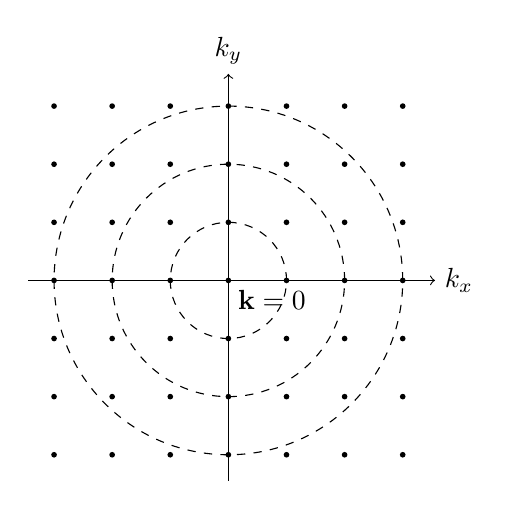
\begin{tikzpicture}[scale=0.82]
\draw[->] (-3.1,0) -- (3.2,0) node[right] {$k_x$};
\draw[->] (0,-3.1) -- (0,3.2) node[above] {$k_y$};
\draw[dashed] (0,0) circle (0.9);
\draw[dashed] (0,0) circle (1.8);
\draw[dashed] (0,0) circle (2.7);
\foreach \x in {-3,-2,-1,0,1,2,3}{
  \foreach \y in {-3,-2,-1,0,1,2,3}{
    \fill (0.9*\x,0.9*\y) circle (1.25pt);
  }
}
\node[below right] at (0,0) {$\mathbf{k}=0$};
\end{tikzpicture}
\caption{有限周期盒子中粒子的离散动量态和等能壳层。}
\end{figure}

对于非相对论粒子，
\begin{equation}
E_{\mathbf{k}}=\frac{\mathbf{k}^2}{2m},
\end{equation}
所以最低能量的态是\(\mathbf{k}=0\)。将\(N\)个全同玻色子放入盒子中，并寻找多粒子基态。第一个玻色子进入零动量态。第二个可以进入同一个态，第三个以及每一个后续玻色子也可以。因此所有\(N\)个玻色子都占据\(\mathbf{k}=0\)。

这是一种玻色子凝聚体：大量全同粒子占据同一个单粒子态，在这里就是最低能态。零动量波函数在空间中是常数，并延伸到整个盒子。它并不把任何一个玻色子定域在某个特定位置上；相应地，每个玻色子都对其所在位置不确定。当占据数变得很大时，共同的波函数会积累出宏观的场振幅，场的行为也越来越像经典场。

费米子基态则完全不同。暂时忽略自旋，于是每个动量点代表一个可用的态。第一个费米子进入\(\mathbf{k}=0\)，但第二个全同费米子不能加入其中。接下来的粒子必须占据能量次低的壳层。在二维图中，有四个最近邻的等能量非零点阵点；在三维中则有六个。这些态被占据之后，进一步的粒子必须进入相继的壳层。

由于能量正比于动量空间中到原点距离的平方，要使总能量最小，就要在泡利不相容原理允许的范围内，让被占据的点尽可能紧密地围绕\(\mathbf{k}=0\)排列。当费米子很多时，被占据的区域近似为一个球。它的边界是费米面，内部是费米海，而整个被填满的区域是费米球。在有限体积下，由于可用的点构成点阵，边界会略微参差不齐，但对于大系统而言这一细节可以忽略。

\begin{figure}
\centering
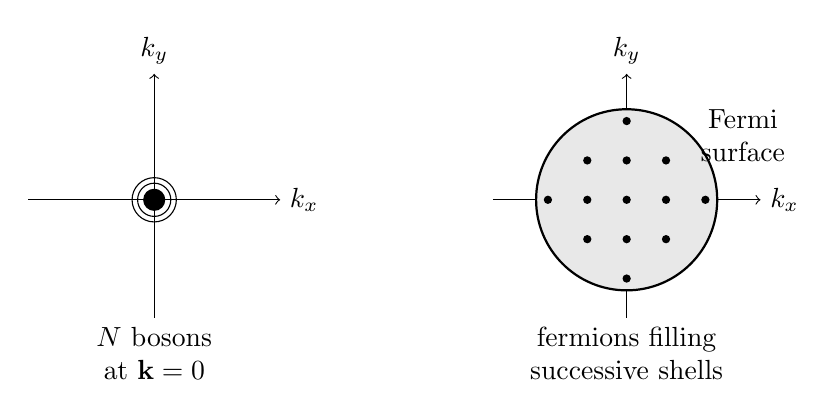
\begin{tikzpicture}[scale=1.0]
\begin{scope}[xshift=-3.0cm]
\draw[->] (-1.6,0) -- (1.6,0) node[right] {$k_x$};
\draw[->] (0,-1.5) -- (0,1.6) node[above] {$k_y$};
\fill (0,0) circle (4pt);
\draw (0,0) circle (6pt);
\draw (0,0) circle (8pt);
\node[align=center] at (0,-1.95) {$N$ bosons\\at $\mathbf{k}=0$};
\end{scope}
\begin{scope}[xshift=3.0cm]
\draw[->] (-1.7,0) -- (1.7,0) node[right] {$k_x$};
\draw[->] (0,-1.5) -- (0,1.6) node[above] {$k_y$};
\fill[gray!18] (0,0) circle (1.15);
\draw[thick] (0,0) circle (1.15);
\fill (0,0) circle (1.5pt);
\fill (0.5,0) circle (1.5pt);
\fill (-0.5,0) circle (1.5pt);
\fill (0,0.5) circle (1.5pt);
\fill (0,-0.5) circle (1.5pt);
\fill (0.5,0.5) circle (1.5pt);
\fill (0.5,-0.5) circle (1.5pt);
\fill (-0.5,0.5) circle (1.5pt);
\fill (-0.5,-0.5) circle (1.5pt);
\fill (1,0) circle (1.5pt);
\fill (-1,0) circle (1.5pt);
\fill (0,1) circle (1.5pt);
\fill (0,-1) circle (1.5pt);
\node[right,align=center] at (0.82,0.82) {Fermi\\surface};
\node[align=center] at (0,-1.95) {fermions filling\\successive shells};
\end{scope}
\end{tikzpicture}
\caption{玻色子凝聚到零动量态，而费米子则向外填充动量态直至费米面。}
\end{figure}

费米子基态的能量比相应的玻色子基态高得多。所有玻色子都可以留在零动量处，但大多数费米子被迫进入非零动量态。随着加入的费米子越来越多，被占据的最大动量也随之增大。此外，大动量处的壳层比原点附近的壳层包含更多的点阵点。因此，一个大的费米球中包含许多处于可观动量的粒子，而只有少数粒子处于最低动量态。

这种对比在激发态中继续存在。对于玻色子，第一激发态是通过从凝聚体中取出任意一个玻色子，并将其放入第一激发单粒子态而得到的：
\begin{equation}
(N,0,0,\ldots)\longrightarrow (N-1,1,0,\ldots).
\end{equation}
移动的是哪一个玻色子并无区别；粒子是全同的。更高的激发可以通过几种方式产生。取决于能级间距，可以把一个玻色子放入更高的能级，也可以把两个玻色子放入第一激发能级。激发玻色子系统意味着把粒子从凝聚体中提升到更高能量的态。

对于费米子，不能把任何粒子移动到已填满的费米球内部的另一个点，因为每一个这样的点都已被占据。从费米海深处取出一个费米子并将其放到费米面之上是可能的，但这需要付出很大的能量。代价最小的激发是从紧靠费米面内侧取出一个费米子，并将其移动到紧靠费米面外侧的一个未被占据的态。被提升的电子在费米面之上只有很小的能量，而留下的空态则在费米面之下只有很小的能量。

\begin{figure}
\centering
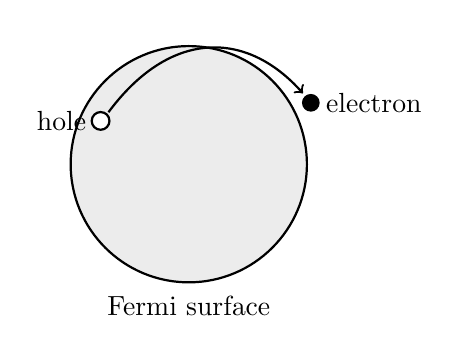
\begin{tikzpicture}[scale=1.0]
\fill[gray!15] (0,0) circle (1.5);
\draw[thick] (0,0) circle (1.5);
\draw[fill=white,thick] (-1.12,0.55) circle (3.2pt);
\fill (1.55,0.78) circle (3.2pt);
\draw[->,thick] (-1.02,0.66) .. controls (-0.25,1.7) and (0.72,1.72) .. (1.45,0.9);
\node[left] at (-1.18,0.55) {hole};
\node[right] at (1.62,0.78) {electron};
\node[below] at (0,-1.55) {Fermi surface};
\end{tikzpicture}
\caption{低能费米子激发使一个电子穿过费米面，并在其后方留下一个空穴。}
\end{figure}

\section{空穴与低能激发}

为了使空穴的电荷具体化，设想盒子中包含均匀弥散在其体积中的正电荷。在物质中，这种正电荷最终来自原子核中的质子，但均匀分布使模型保持简单。加入足够多的电子以使背景中和。在基态中，这些电子填满费米球。

把一个电子从费米面之下提升到费米面之上，并不会改变盒子的总电荷。它在费米面之上产生一个带负电的电子，并在费米面之下留下一个缺失的负电荷。因此，缺失的电子可以被当作一个带正电的激发：空穴。

\begin{classroomqa}
\lecturetimestamp{01:31:38}
\audiencequestion{费米面之下的空穴具有负能量吗？}
\lecturerresponse{不。空穴是多体基态之上的一个激发，因此其激发能是正的。当能量相对于费米面来度量时，从费米面之下移走一个被占据的电子需要付出正的能量。}
\end{classroomqa}

设被移走的电子具有能量 \(\varepsilon<\varepsilon_F\)，被激发的电子具有能量 \(\varepsilon'>\varepsilon_F\)。所提供的能量可以分解为两个相对于费米面的正距离。\footnote{这两个间隔是分别陈述的；此处展示的紧凑等式是代数上等价的重新构造。}
\begin{equation}
\Delta E
=\varepsilon'-\varepsilon
=(\varepsilon'-\varepsilon_F)+(\varepsilon_F-\varepsilon).
\end{equation}
第一项贡献自然地归属于费米面以上的电子，而第二项则归属于其下方的空穴：
\begin{equation}
E_{\mathrm{electron}}=\varepsilon'-\varepsilon_F>0,
\qquad
E_{\mathrm{hole}}=\varepsilon_F-\varepsilon>0.
\end{equation}
电子带负电荷，空穴带正电荷。

费米面以上的电子随后可能落入一个可用的空穴。此时其能量降低，因此辐射必须将释放的能量带走。人们可以将该事件描述为一个电子落入一个未被占据的较低能态并发射一个或多个光子。等价地，也可以说一个电子和一个空穴湮灭为辐射。空穴并不是盒中额外的基本组分；它是被填充的多电子态中的一个缺失。尽管如此，它的能量和电荷使得将其视为一种类粒子激发是有用的。

\begin{classroomqa}
\lecturetimestamp{01:36:52}
\audiencequestion{激发一个电子是否意味着在动量空间中将其从一个格点移动到另一个格点？}
\lecturerresponse{它意味着将电子从一个能级移动到另一个能级。对于盒中的自由粒子，动量点阵标记这些能级，但同样的想法并不依赖于动量空间点阵。在原子中，正电荷集中在原子核内。电子填充最低的可用原子能级，而一个光子可以将一个电子激发到激发能级，并在其原来所在的能级中留下一个空位。该空位就是空穴在原子中的对应物。}
\end{classroomqa}

在盒中，光子吸收同样将光子能量转化为费米面以上的一个电子和其下方的一个空穴。在原子中，同样的语言描述被激发的电子以及在被占据的较低能级中留下的空位。

\begin{classroomqa}
\lecturetimestamp{01:39:16}
\audiencequestion{低能光子能否被费米球中任意位置的电子吸收？}
\lecturerresponse{不能。如果电子位于费米海深处，其附近的所有态都已被占据，低能光子无法将其一直提升到费米面以上的未占据态。只有足够靠近费米面的电子，才在光子能量范围内具有可及的空态。能量足够高的光子可以将电子从费米海深处激发出来。}
\end{classroomqa}

因此，低能吸收截面由费米海的表面而非其整个体积决定。费米海深处的电子被阻止发生小跃迁；而紧邻费米面下方的电子则可以被移动到紧邻其上方。

\begin{classroomqa}
\lecturetimestamp{01:40:42}
\audiencequestion{是什么阻止了电子在没有入射光子的情况下直接相互作用？}
\lecturerresponse{没有任何东西。在这个简单模型中，电子--电子相互作用被忽略，因为将其包括进来会使费米海图像变得更加复杂。在对金属的这一初步近似中，它们的有效影响被视为足够弱，以至于通常可以忽略。}
\end{classroomqa}

\begin{classroomqa}
\lecturetimestamp{01:41:10}
\audiencequestion{如果一个光子携带足够的能量来激发多个电子，会发生什么？}
\lecturerresponse{任何与守恒定律一致的过程原则上都是可能的。光子可以产生多于一个电子--空穴对：激发两个电子也会留下两个空穴。这样的过程产生更多激发，并且通常比将能量用于更强烈地激发一个电子的概率更低。}
\end{classroomqa}

\begin{classroomqa}
\lecturetimestamp{01:42:06}
\audiencequestion{当两个光子各自单独都不能产生激发时，它们能否被一起吸收？}
\lecturerresponse{能。吸收是概率性的，当两个光子的能量之和达到一个可用的激发时，即使其中任一光子单独都低于所需能量，双光子过程也可以发生。如果可用的光所携带的能量太少，无法达到任何允许的激发，那么它基本上会穿过该系统。}
\end{classroomqa}

\editorialnote{此处有一段简短讨论将吸收辐射与集体电子运动联系起来，但其实质性细节无法复原。唯一可靠的是如下陈述：这种集体响应比单粒子--空穴图像更为复杂。}

\begin{classroomqa}
\lecturetimestamp{01:43:49}
\audiencequestion{为什么电子--电子相互作用被称为弱相互作用，尽管所有电子都带相同的负电荷？}
\lecturerresponse{电子浸没在起补偿作用的正电荷背景中。该背景屏蔽了电子的电荷，并在这个简化设定中减弱了有效相互作用。相互作用并非不存在；处理它需要考虑介质的屏蔽响应。}
\end{classroomqa}

\begin{classroomqa}
\lecturetimestamp{01:44:41}
\audiencequestion{屏蔽效应会在后面讨论吗？}
\lecturerresponse{是的。屏蔽效应很重要，但它被推迟到能够更完整地处理相互作用体系时再讨论。}
\end{classroomqa}

\section{一维费米海与反粒子}

空穴构造指向反粒子。同样的逻辑结构可以从物质中的电子转移到相对论量子场及其真空。最简单的版本使用一个空间维度和一个无质量费米场 \(\psi(x,t)\)。在光速取为1的单位制中，两种可能的线性色散关系为
\begin{equation}
\omega=k,
\qquad\text{or}\qquad
\omega=-k.
\end{equation}
我们将明确考虑第一个分支。

\editorialnote{结尾的交流交替使用了互不相容的粒子识别。可靠的模型是一个未指定的、无质量的、位于一个空间维度中的费米玩具场，且只限于一个传播方向。}

对于平面波
\begin{equation}
\psi(x,t)=e^{i(kx-\omega t)},
\end{equation}
其导数为
\begin{equation}
\frac{\partial\psi}{\partial t}=-i\omega\psi,
\qquad
\frac{\partial\psi}{\partial x}=ik\psi.
\end{equation}
因此 \(\omega=k\) 等价于一阶场方程
\begin{equation}
\frac{\partial\psi}{\partial t}
=-\frac{\partial\psi}{\partial x}.
\end{equation}

\begin{figure}
\centering
\includegraphics[width=0.72\textwidth]{lecture_05_figure_05.png}
\caption{开始讨论其平面波满足 \(\omega=k\) 的一阶场方程。}
\lectureframe{01:47:22}
\end{figure}

任何形如 \(f(x-t)\) 的剖面都满足这个方程并向右移动。改变符号则得到
\begin{equation}
\frac{\partial\psi}{\partial t}
=+\frac{\partial\psi}{\partial x},
\end{equation}
其剖面 \(f(x+t)\) 向左移动。任一阶方程都只选择一个运动方向。取该场为费米场，并且为了空穴论证，假设其粒子带电荷。

分支 \(\omega=k\) 立即带来一个困难。波数 \(k\) 可以为负，因此 \(\omega\) 也可以为负。由于在这些单位中 \(\omega\) 就是能量，直线谱同时包含正能量态和负能量态：
\begin{equation}
E=\omega=k.
\end{equation}

\begin{figure}
\centering
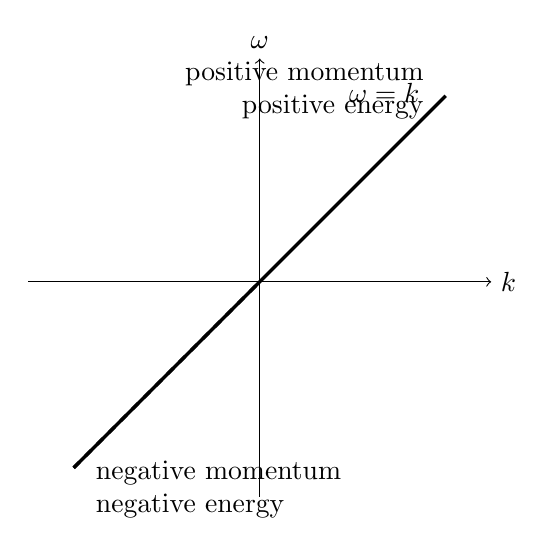
\begin{tikzpicture}[scale=1.05]
\draw[->] (-2.8,0) -- (2.8,0) node[right] {$k$};
\draw[->] (0,-2.6) -- (0,2.7) node[above] {$\omega$};
\draw[very thick] (-2.25,-2.25) -- (2.25,2.25);
\draw[very thick,dashed] (-2.25,-2.25) -- (0,0);
\node[above left] at (2.05,2.05) {$\omega=k$};
\node[below right,align=left] at (-2.1,-2.05) {negative momentum\\negative energy};
\node[above left,align=right] at (2.1,1.85) {positive momentum\\positive energy};
\end{tikzpicture}
\caption{单分支谱 \(\omega=k\)，其负能量半支位于 \(k<0\)。}
\end{figure}

普通的空真空不可能是这种理论的基态。一个正能量费米子可以辐射一个光子并跃迁到更低的状态。没有什么会迫使它在零处停下：它可以继续进入负能量态，发射更多辐射，并无限制地向下跃迁。费米子失去的能量会出现在辐射场中。因此，一个下方无界的谱不会给出稳定的普通真空。

费米子排他性提供了另一个出发点。将每一个负能量单粒子态，直到零能量为止，都填入一个费米子。没有其他费米子能落入这些态，因为每一个态都已被占据。再添加一个负能量费米子是不可能的，而添加一个正能量费米子则会提高能量。因此，完全填满的负能量海可以被取为多体基态，并称为真空。

\begin{figure}
\centering
\resizebox{\linewidth}{!}{%
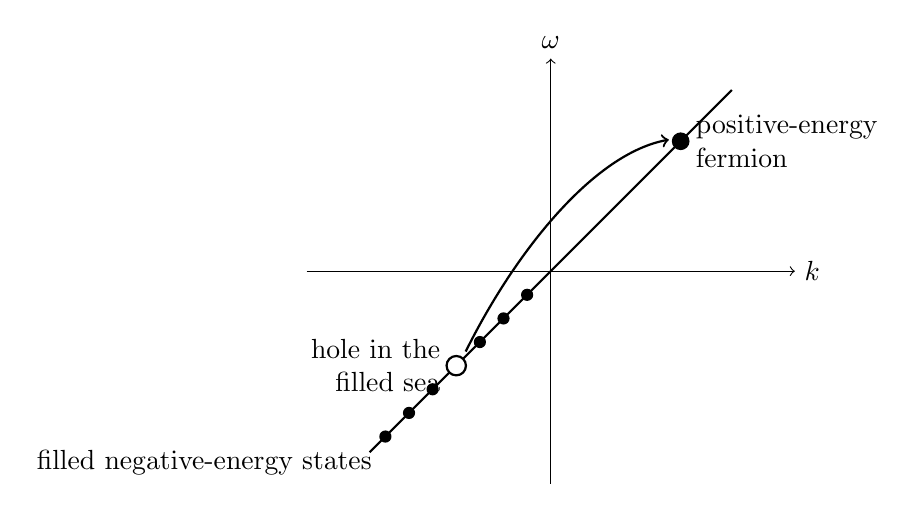
\begin{tikzpicture}[scale=1.0]
\draw[->] (-3.1,0) -- (3.1,0) node[right] {$k$};
\draw[->] (0,-2.7) -- (0,2.7) node[above] {$\omega$};
\draw[thick] (-2.3,-2.3) -- (2.3,2.3);
\foreach \p in {-2.1,-1.8,-1.5,-1.2,-0.9,-0.6,-0.3}{
  \fill (\p,\p) circle (2.2pt);
}
\draw[fill=white,thick] (-1.2,-1.2) circle (3.5pt);
\fill (1.65,1.65) circle (3.2pt);
\draw[->,thick] (-1.08,-1.02) .. controls (-0.45,0.25) and (0.55,1.5) .. (1.5,1.67);
\node[left,align=right] at (-1.28,-1.2) {hole in the\\filled sea};
\node[right,align=left] at (1.72,1.65) {positive-energy\\fermion};
\node[below left] at (-2.15,-2.15) {filled negative-energy states};
\end{tikzpicture}%
}
\caption{填满的负能量海，以及通过将一个费米子激发到正能量而形成的激发。}
\end{figure}

最简单的激发是从负能量海中移走一个费米子，并将其放入一个正能量态。被激发的费米子是一个普通的正能量粒子。海中留下的空位是第二种激发，即空穴。如果被移走的费米子带负电荷，那么空穴带正电荷。

在这个单分支例子中，空穴也具有正动量。如果缺失的费米子原本占据动量为 \(k_-<0\) 的态，那么移走它会使总动量改变
\begin{equation}
p_{\mathrm{hole}}=-k_->0.
\end{equation}
这是负动量的缺失。因此，该激发由一个正能量、带负电的费米子和一个正能量、带正电的空穴组成。二者都携带正动量，并且在 \(\omega=k\) 分支上，二者都向右移动。

在完整的电子理论中，带正电的空穴就是正电子。狄拉克最初考虑将空穴等同于质子。该构造要求一个粒子与其反粒子具有相同的质量。空穴是一种不同的粒子，具有电子的质量和相反的电电荷。这就是负能量谱所导致的基本粒子--反粒子解释。

同样的补救办法不能应用于玻色子。一个玻色子态允许任意多个粒子，因此无法将某个负能级填充一次就阻止其进一步被占据。总可以向该能级添加更多玻色子，一次又一次地降低能量：
\begin{equation}
\begin{aligned}
\text{fermionic mode: }&n=0\ \text{or}\ 1,\\
\text{bosonic mode: }&n=0,1,2,\ldots .
\end{aligned}
\end{equation}
所提出的玻色子系统仍将没有基态。在这一初等构造中，填满的海的稳定性恰恰依赖于费米子排斥。

这个一维方程只是狄拉克方程的一个玩具版本。它的场是无质量的，以光速运动，并且只沿一个方向传播。一个更完整的狄拉克方程必须容纳缺失的运动方向以及相对论性粒子结构的其余部分。那个更完整的方程，连同玻色子场的反粒子处理，都推迟到以后讨论。
